\documentclass[11pt,a4paper]{article}
% ---------------------------------------------------------------------------
% Shared preamble: page geometry, typography, colours, table and code styles.
% ---------------------------------------------------------------------------
\usepackage[T1]{fontenc}
\usepackage[utf8]{inputenc}
\usepackage{lmodern}
\usepackage[a4paper,margin=27mm,top=25mm,bottom=28mm]{geometry}
\usepackage{microtype}
% Let TeX stretch the last resort rather than overflow the margin: long
% \texttt{} tokens (flag names, identifiers) cannot be hyphenated.
\setlength{\emergencystretch}{3em}
\hyphenpenalty=1000
\tolerance=1200
\usepackage{booktabs}
\usepackage{tabularx}
\usepackage{array}
\usepackage{graphicx}
\usepackage{xcolor}
\usepackage{amsmath}
\usepackage{enumitem}
\usepackage{caption}
\usepackage{fancyhdr}
\usepackage{titlesec}
\usepackage{listings}
\usepackage{tikz}
\usepackage[hidelinks]{hyperref}
\usetikzlibrary{arrows.meta,positioning,fit,backgrounds}

% -- palette (matches the figures the tool generates) -----------------------
\definecolor{accent}{HTML}{2A78D6}
\definecolor{ink}{HTML}{0B0B0B}
\definecolor{inksoft}{HTML}{52514E}
\definecolor{rule}{HTML}{E4E3DF}
\definecolor{band}{HTML}{F5F7FA}
\definecolor{warn}{HTML}{D03B3B}

% -- headings ---------------------------------------------------------------
\titleformat{\section}{\Large\bfseries\color{accent}}{\thesection}{0.7em}{}
\titleformat{\subsection}{\large\bfseries\color{ink}}{\thesubsection}{0.7em}{}
\titleformat{\subsubsection}{\normalsize\bfseries\color{inksoft}}{\thesubsubsection}{0.7em}{}
\titlespacing*{\section}{0pt}{2.2ex plus 1ex minus .2ex}{1.2ex plus .2ex}

% -- running heads ----------------------------------------------------------
\pagestyle{fancy}
\fancyhf{}
\renewcommand{\headrulewidth}{0.4pt}
\renewcommand{\footrulewidth}{0pt}
\fancyhead[L]{\footnotesize\color{inksoft}OmniCLF --- Technical Report}
\fancyhead[R]{\footnotesize\color{inksoft}\leftmark}
\fancyfoot[C]{\footnotesize\color{inksoft}\thepage}

% -- float placement --------------------------------------------------------
% Defaults strand wide figures on pages of their own; let floats share a page
% with a decent amount of text instead.
\renewcommand{\topfraction}{0.92}
\renewcommand{\bottomfraction}{0.75}
\renewcommand{\textfraction}{0.07}
\renewcommand{\floatpagefraction}{0.80}
\setcounter{topnumber}{2}
\setcounter{totalnumber}{3}

% -- captions ---------------------------------------------------------------
\captionsetup{font=small,labelfont={bf,color=accent},width=.92\textwidth}

% -- tables -----------------------------------------------------------------
\renewcommand{\arraystretch}{1.25}
\newcolumntype{L}[1]{>{\raggedright\arraybackslash}p{#1}}
% Ragged-right inside X columns: justifying short table prose opens ugly
% inter-word gaps in a narrow measure.
\renewcommand{\tabularxcolumn}[1]{>{\raggedright\arraybackslash}p{#1}}
\newcolumntype{R}[1]{>{\raggedleft\arraybackslash}p{#1}}
\newcommand{\best}[1]{\textbf{#1}}

% -- code -------------------------------------------------------------------
\lstdefinestyle{py}{
  language=Python,
  basicstyle=\ttfamily\footnotesize,
  keywordstyle=\color{accent},
  commentstyle=\color{inksoft}\itshape,
  stringstyle=\color{inksoft},
  numbers=none,
  frame=leftline,
  framerule=1.6pt,
  rulecolor=\color{rule},
  xleftmargin=10pt,
  framexleftmargin=10pt,
  breaklines=true,
  showstringspaces=false,
  aboveskip=1.1em, belowskip=1.1em,
}
\lstdefinestyle{sh}{
  language=bash,
  basicstyle=\ttfamily\footnotesize,
  keywordstyle=\color{ink},
  numbers=none,
  frame=leftline, framerule=1.6pt, rulecolor=\color{rule},
  xleftmargin=10pt, framexleftmargin=10pt,
  breaklines=true, showstringspaces=false,
  aboveskip=1.1em, belowskip=1.1em,
}
\lstset{style=py}

% -- callout box ------------------------------------------------------------
\newcommand{\keypoint}[1]{%
  \begin{center}
  \begin{minipage}{0.94\textwidth}
    \setlength{\fboxsep}{9pt}%
    \colorbox{band}{\begin{minipage}{\dimexpr\textwidth-2\fboxsep}
      \small #1
    \end{minipage}}
  \end{minipage}
  \end{center}
}


\begin{document}

% ===========================================================================
% Title
% ===========================================================================
\begin{titlepage}
\centering
\vspace*{2.2cm}

{\color{accent}\rule{\textwidth}{2pt}}\\[1.1em]
{\Huge\bfseries OmniCLF\par}
\vspace{0.7em}
{\LARGE An All-in-One, Leakage-Free Pipeline\\[0.3em] for Tabular Classification\par}
\vspace{0.9em}
{\color{accent}\rule{\textwidth}{2pt}}

\vspace{2.2cm}
{\large Technical Report\par}
\vspace{0.4em}
{\large Version 2.0\par}
\vspace{2.6cm}

\begin{minipage}{0.86\textwidth}
\small
\setlength{\parskip}{0.7em}\setlength{\parindent}{0pt}
\textbf{Abstract.} Automated machine-learning tools are easy to write and easy
to get wrong. The usual failure is not a poorly chosen model but a \emph{leaky
evaluation}: a scaler, an imputer or a feature ranking fitted on the whole
dataset before the validation folds are drawn, so that every reported score is
quietly optimistic and nothing in the output reveals it. This report documents
OmniCLF, a command-line tool that turns an arbitrary tabular CSV into a
complete, reproducible classification experiment, and the engineering decisions
that make its numbers defensible.

Three properties define the system. First, every data-dependent transformation
is a stage of a single scikit-learn \texttt{Pipeline} and is therefore refitted
from scratch inside each training fold, which makes preprocessing leakage
structurally impossible rather than merely discouraged. Second, models are
ranked by macro $F_1$ with balanced accuracy and Matthews' correlation
coefficient reported alongside, because on imbalanced targets plain accuracy
rewards degenerate classifiers. Third, every run writes the configuration that
produced it, so any number in any report can be regenerated with one command.

The tool is evaluated on a demographic and health survey extract of 30{,}548
records with a $4.89\!:\!1$ class ratio, benchmarking eight classifiers. The
result illustrates the motivation better than any argument: the model with the
highest accuracy in the table, $83.0\%$, is a degenerate majority-class
predictor with a balanced accuracy of exactly $0.500$ and a \emph{negative}
MCC. It ranks first by the metric the previous version of this project
reported, and last by every metric that respects the minority class.
\end{minipage}

\vfill
{\small\color{inksoft} September 2026}
\end{titlepage}

\tableofcontents
\newpage

% ===========================================================================
\section{Introduction}
\markboth{Introduction}{}

\subsection{Problem statement}

Given an arbitrary tabular dataset with a categorical target, produce (i)~an
unbiased estimate of how well a classifier would perform on data it has never
seen, and (ii)~a report a reader can audit without reading the source code.

The emphasis belongs on \emph{unbiased}. A tool that returns optimistic numbers
is worse than no tool at all, because the optimism is invisible in the output:
a leaked accuracy of $0.94$ looks exactly like an honest accuracy of $0.94$.
The practitioner has no signal that anything is wrong, and the error surfaces
only in production, or in review, or never.

\subsection{Scope}

OmniCLF handles binary and multi-class classification on tabular data of the
size that fits in memory---roughly up to a few hundred thousand rows. It does
not attempt neural architecture search, does not handle images, text or
sequences, and deliberately offers small hyper-parameter grids: the
contribution is methodological correctness, not leaderboard performance.

\subsection{Design goals}

\begin{center}
\begin{tabularx}{\textwidth}{L{4.1cm} X}
\toprule
\textbf{Goal} & \textbf{How it is met} \\
\midrule
Correct by construction & leakage is prevented by the object graph, not by the user remembering to do the right thing \\
Honest by default & the ranking metric respects class imbalance; misleading metrics are shown but never used to rank \\
Reproducible & one seed, one configuration file, one command to replay \\
Auditable & per-fold scores, library versions and the full log are written to disk, not just summary means \\
Extensible & a new technique is one row in a registry table \\
Backward compatible & \texttt{python main.py} still runs the original guided menu flow \\
\bottomrule
\end{tabularx}
\end{center}

% ===========================================================================
\section{Background: why reported accuracy is usually too high}
\markboth{Background}{}

Four failure modes account for most of the gap between reported and realised
performance in applied classification work. The architecture in
Section~\ref{sec:design} is arranged to exclude each one.

\subsection{Preprocessing leakage}
\label{sec:leakage}

Scaling constants, imputation values, encoder vocabularies and feature rankings
are all \emph{learned} from data; they are model parameters wearing a different
hat. If they are learned once from the whole dataset and the data is then split
into folds, each fold's validation rows have already influenced the
transformation applied to its training rows. Information has crossed a boundary
the evaluation assumes is sealed.

The size of the effect depends on the transformation:

\begin{center}
\begin{tabularx}{\textwidth}{L{4.4cm} L{2.6cm} X}
\toprule
\textbf{Transformation} & \textbf{Typical bias} & \textbf{Why} \\
\midrule
Centring / scaling & small & two moments estimated from many rows are stable \\
Imputation & small--moderate & grows as missingness grows \\
\textbf{Supervised feature selection} & \textcolor{warn}{\textbf{large}} & choosing $k$ of $p$ features on the full sample can manufacture apparent signal from pure noise when $p \gg k$ \\
Resampling (SMOTE etc.) & \textcolor{warn}{large} & synthetic training points interpolated from validation rows \\
\bottomrule
\end{tabularx}
\end{center}

The feature-selection case is the dangerous one, and it is precisely what an
automated tool is most likely to do, because selection is expensive and caching
it outside the fold loop is the obvious optimisation. Hastie et
al.~\cite{esl} devote a section of \emph{The Elements of Statistical Learning}
to exactly this, under the heading ``the wrong way to do cross-validation'',
and demonstrate a $3\%$ error rate on data containing no signal at all.

\subsection{Inconsistent feature spaces}
\label{sec:spaces}

A subtler variant, and one that static analysis will not catch: fitting the
transformers \emph{separately} on the training and test matrices.

\begin{lstlisting}
X_train_scaled = scaler.fit_transform(X_train)
X_test_scaled  = scaler.fit_transform(X_test)   # a second, different scaler
\end{lstlisting}

Both matrices have the right shape. No exception is raised. Every downstream
call works. But the two scalers learned different means and variances, so
column $k$ of the test matrix no longer denotes the same quantity as column $k$
of the training matrix, and the model is asked to interpret a feature vector in
a coordinate system it was never trained in. The resulting test score is not
biased in a predictable direction---it is simply meaningless. If the same
mistake is made with a \emph{supervised} selector, the two matrices may not
even contain the same features.

\subsection{Accuracy on an imbalanced target}
\label{sec:imbalance}

For a target whose majority class has prevalence $\pi$, the constant classifier
``always predict the majority'' achieves accuracy $\pi$ while learning nothing.
On the dataset used here $\pi = 0.83$. Any model reporting accuracy below
$0.83$ is, on that metric alone, worse than a single \texttt{return} statement,
and any model slightly above it may be doing almost nothing.

Accuracy also hides \emph{which} errors are made, which is usually the
decision-relevant question. Screening for an intervention cares about recall on
the minority class; the majority class is not the point of the exercise.

\subsection{Reading a difference that is not there}

With five folds, a $0.004$ difference in mean macro $F_1$ between two models
sits well inside fold-to-fold noise. A table of bare means nonetheless invites
the reader to declare a winner, and the winner will often change if the seed
changes.

% ===========================================================================
\section{Audit of the previous implementation}
\markboth{Audit of v1}{}

Version~1 of this project (December 2023) was a 154-line script plus four
interactive helper modules: \texttt{normalization.py},
\texttt{feature\_selection.py}, \texttt{cross\_val.py} and \texttt{modals.py}.
It ran, it produced a PDF, and it exhibited three of the four failure modes
above. The defects are documented here because the rewrite is organised around
them, and because they are ordinary mistakes rather than exotic ones.

\subsection{Defect 1 --- separately fitted transformers}

\begin{lstlisting}
# v1/normalization.py
def scaling(df1, df2):
    ...
    normalized_df   = scaler.fit_transform(df1)   # training set
    normalized_df_b = scaler.fit_transform(df2)   # hold-out set, refitted
    return normalized_df, normalized_df_b
\end{lstlisting}

The hold-out set received its own independently fitted scaler
(\S\ref{sec:spaces}). The same pattern appeared in the selector, with an
additional consequence:

\begin{lstlisting}
# v1/feature_selection.py
X = selector.fit_transform(scaled_data, y)
y = selector.fit_transform(scaled_data_blind, y_blind)  # a feature matrix, named y
return X, y
\end{lstlisting}

A second selector was fitted on the hold-out set, and because feature ranking
is data-dependent it could select a \emph{different subset of features}. The
variable name \texttt{y} for a feature matrix is a symptom of the confusion,
not its cause.

\subsection{Defect 2 --- preprocessing outside the fold loop}

\begin{lstlisting}
# v1/main.py
scaled_data, scaled_data_blind = scaling(X, X_blind)
X_reduced, X_reduced_blind     = feature_selection(scaled_data, y, ...)
accuracy_scores = cross_val_score(classifier, X_reduced, y, cv=kf, ...)
\end{lstlisting}

Scaling and ANOVA-based selection ran \emph{once}, on the whole training set,
before \texttt{cross\_val\_score} drew any folds (\S\ref{sec:leakage}). Every
fold's validation rows had therefore already participated in choosing which
features the model would see.

\subsection{Defect 3 --- accuracy-only reporting}

The PDF contained accuracy, macro precision, macro recall and macro $F_1$ per
fold, but the console output, the plots and the narrative were all built around
accuracy, on a target where the constant classifier scores $83\%$
(\S\ref{sec:imbalance}).

\subsection{Secondary issues}

\begin{itemize}[leftmargin=1.4em,itemsep=0.25em]
  \item \texttt{X = data.iloc[:, 1:-1]} silently discarded the first column of every dataset.
  \item \texttt{data.fillna(data.mode().iloc[0])} imputed using a mode computed over the whole dataset, including the hold-out rows---a third leakage path.
  \item \texttt{pd.factorize} assigned arbitrary integers to nominal categories, imposing a false ordering on unordered values such as region names.
  \item \texttt{log\_data = X.apply(np.log1p)} was computed and never used; on negative inputs it would have produced \texttt{NaN} silently.
  \item Selecting Group $k$-fold crashed, because no grouping vector was ever passed.
  \item The PDF placed every string at a hand-computed canvas coordinate, so the layout collapsed whenever the number of folds or metrics changed.
\end{itemize}

\subsection{What was kept}

The rewrite deliberately preserves what v1 got right: the four-way
decomposition into scaling / selection / validation / model, the menu of
techniques under each, and the guided interactive flow. \texttt{python main.py}
with no arguments still asks the same questions in the same order. The registry
tables of Section~\ref{sec:registries} \emph{are} those menus, promoted from
\texttt{if}/\texttt{elif} chains to data.

% ===========================================================================
\section{System design}
\label{sec:design}
\markboth{System design}{}

\subsection{Architecture}

\begin{figure}[htbp]
\centering
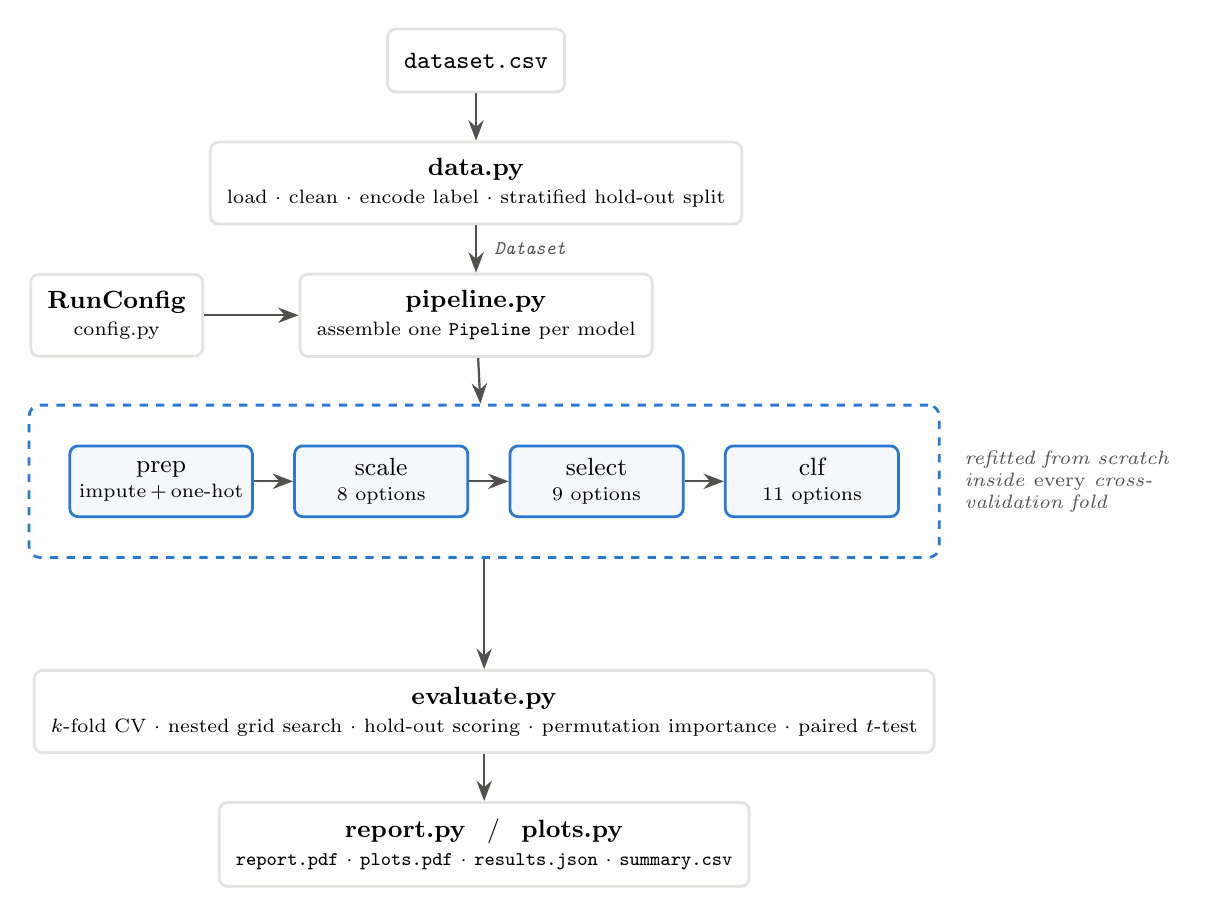
\begin{tikzpicture}[
  font=\small,
  node distance=6mm,
  box/.style={draw=rule,line width=1pt,rounded corners=3pt,fill=white,
              minimum height=8mm,inner sep=6pt,align=center},
  stage/.style={draw=accent,line width=1pt,rounded corners=3pt,fill=band,
                minimum height=9mm,minimum width=22mm,align=center},
  note/.style={font=\scriptsize\itshape,color=inksoft},
  arrow/.style={-{Stealth[length=2.6mm]},draw=inksoft,line width=0.8pt},
]
\node[box] (csv) {\texttt{dataset.csv}};
\node[box,below=of csv] (data) {\textbf{data.py}\\[-1pt]{\scriptsize load $\cdot$ clean $\cdot$ encode label $\cdot$ stratified hold-out split}};
\node[box,below=of data] (pipe) {\textbf{pipeline.py}\\[-1pt]{\scriptsize assemble one \texttt{Pipeline} per model}};

\node[stage,below=11mm of pipe,xshift=-40mm] (prep) {prep\\[-2pt]{\scriptsize impute\,+\,one-hot}};
\node[stage,right=5mm of prep] (scale) {scale\\[-2pt]{\scriptsize 8 options}};
\node[stage,right=5mm of scale] (select) {select\\[-2pt]{\scriptsize 9 options}};
\node[stage,right=5mm of select] (clf) {clf\\[-2pt]{\scriptsize 11 options}};
\draw[arrow] (prep) -- (scale);
\draw[arrow] (scale) -- (select);
\draw[arrow] (select) -- (clf);

\begin{scope}[on background layer]
  \node[draw=accent,dashed,line width=1pt,rounded corners=4pt,
        fit=(prep)(clf),inner sep=5mm] (fold) {};
\end{scope}
\node[note,right=2mm of fold.east,text width=26mm,align=left]
  {refitted from scratch inside \emph{every} cross-validation fold};

\node[box,below=14mm of fold] (eval) {\textbf{evaluate.py}\\[-1pt]{\scriptsize $k$-fold CV $\cdot$ nested grid search $\cdot$ hold-out scoring $\cdot$ permutation importance $\cdot$ paired $t$-test}};
\node[box,below=of eval] (rep) {\textbf{report.py} \, / \, \textbf{plots.py}\\[-1pt]{\scriptsize \texttt{report.pdf} $\cdot$ \texttt{plots.pdf} $\cdot$ \texttt{results.json} $\cdot$ \texttt{summary.csv}}};

\node[box,left=12mm of pipe] (cfg) {\textbf{RunConfig}\\[-1pt]{\scriptsize config.py}};

\draw[arrow] (csv) -- (data);
\draw[arrow] (data) -- node[note,right]{\ \texttt{Dataset}} (pipe);
\draw[arrow] (cfg) -- (pipe);
\draw[arrow] (pipe) -- (fold);
\draw[arrow] (fold) -- (eval);
\draw[arrow] (eval) -- (rep);
\end{tikzpicture}
\caption{The pipeline. Because the four stages are one estimator,
\texttt{cross\_validate} clones and refits all of them on each training fold,
so no statistic learned from validation rows can reach the model.}
\label{fig:arch}
\end{figure}

\begin{center}
\begin{tabularx}{\textwidth}{L{4.15cm} X}
\toprule
\textbf{Module} & \textbf{Responsibility} \\
\midrule
\texttt{config.py} & \texttt{RunConfig} --- the single, JSON-serialisable source of truth \\
\texttt{data.py} & loading, cleaning, schema inference, stratified hold-out split \\
\texttt{preprocessing.py} & scaler registry (was \texttt{normalization.py}) \\
\texttt{feature\_selection.py} & selector registry \\
\texttt{cross\_val.py} & validation-scheme registry \\
\texttt{models.py} & classifier registry with hyper-parameter grids (was \texttt{modals.py}) \\
\texttt{pipeline.py} & assembles \textsf{prep} $\to$ \textsf{scale} $\to$ \textsf{select} $\to$ \textsf{clf} \\
\texttt{evaluate.py} & cross-validation, hold-out scoring, importance, statistical tests \\
\texttt{plots.py} & figures, in one validated visual style \\
\texttt{report.py} & PDF, JSON and CSV artefacts \\
\texttt{runner.py} & orchestration; owns the run directory \\
\texttt{interactive.py} & the guided menu flow from v1 \\
\texttt{cli.py} & argument parsing and the console summary \\
\bottomrule
\end{tabularx}
\end{center}

\subsection{Configuration as the unit of reproducibility}

Every experiment is fully described by a \texttt{RunConfig} dataclass: dataset
path, target, cleaning rules, the four pipeline choices, validation parameters,
seed and output settings. It validates itself on construction
(\texttt{holdout\_size} in range, $\texttt{n\_splits} \ge 2$, at least one
model), serialises to JSON, and rejects unknown keys on load so that a typo in
a hand-edited configuration fails loudly instead of being silently ignored.

The run directory is written \emph{before} the experiment starts, and the
configuration file is the first thing in it. Three consequences follow: a
crashed run still documents what was attempted; \texttt{-{}-config
runs/<name>/config.json} replays a run exactly; and the interactive flow is not
a separate code path---it simply fills the same dataclass the CLI flags fill.

\subsection{The data layer}

\texttt{data.py} performs only \emph{row-independent} work. Anything that
learns a statistic from the data is deferred to the pipeline, where the fold
machinery can control it. Concretely, the loader:

\begin{enumerate}[leftmargin=1.6em,itemsep=0.25em]
  \item \textbf{Disambiguates duplicate headers.} Survey exports repeat column names---this dataset has two columns called ``Anemia level''---which makes every later column selection ambiguous.
  \item \textbf{Drops rows with no label}: missing, blank, and any value named by \texttt{-{}-drop-target-values} (here, \texttt{"Don't know"}). A row without supervision contributes nothing and, if imputed, contributes noise.
  \item \textbf{Drops classes too rare to stratify.} Fewer than two rows cannot be split across folds.
  \item \textbf{Encodes the label} to integers, retaining the original names for reports.
  \item \textbf{Drops unusable columns}: all-missing, constant, or non-numeric with more than 50 distinct values (identifiers and free text).
  \item \textbf{Infers the schema}---numeric versus categorical---and splits off a stratified hold-out set.
\end{enumerate}

Note what is \emph{absent}: no imputation, no encoding, no scaling. Those are
stages of the pipeline.

\subsection{Registries}
\label{sec:registries}

The four v1 modules became declarative tables mapping a key to a label, a
factory and a one-line rationale:

\begin{lstlisting}
SCALERS = {
    "robust": ("RobustScaler", lambda: RobustScaler(),
               "median / IQR scaling; preferred when outliers are present"),
    ...
}
\end{lstlisting}

\begin{center}
\begin{tabularx}{\textwidth}{L{2.4cm} X r}
\toprule
\textbf{Registry} & \textbf{Entries} & \textbf{\#} \\
\midrule
Scalers & Standard, Min--Max, Robust, Normalizer, MaxAbs, Power (Yeo--Johnson), Quantile, none & 8 \\
Selectors & ANOVA $F$-test, mutual information, $F$-statistic, variance threshold, RFE, PCA, L1/LASSO, tree importance, none & 9 \\
Validation & stratified $k$-fold, $k$-fold, repeated stratified, group $k$-fold, time-series split, shuffle split, stratified shuffle & 7 \\
Classifiers & Random Forest, Extra Trees, Histogram Gradient Boosting, Gradient Boosting, Logistic Regression, SVM (RBF), $k$-NN, Gaussian NB, Decision Tree, LDA, MLP & 11 \\
\bottomrule
\end{tabularx}
\end{center}

Adding a technique is one row: the CLI choices, the interactive menu, the
report labels and the parametrised tests all derive from the tables. The
classifier registry additionally carries a small grid per model, keyed
\texttt{clf\_\_*} so it can be handed straight to \texttt{GridSearchCV} over the
pipeline, and a \texttt{\_SUPPORTS\_CLASS\_WEIGHT} set so that
\texttt{class\_weight="balanced"} is applied exactly where the estimator
accepts it.

One non-obvious constraint: registry factories must produce \emph{picklable}
estimators, because joblib pickles them to ship to worker processes when
\texttt{n\_jobs > 1}. The mutual-information selector therefore wraps its
scoring function in \texttt{functools.partial} rather than a lambda---a mistake
that manifests only under parallelism, and so is pinned by a test.

\subsection{The pipeline}

\begin{lstlisting}
Pipeline([
    ("prep",   ColumnTransformer([...])),   # impute + one-hot encode
    ("scale",  build_scaler(config.scaler)),
    ("select", build_selector(config.selector, k, seed)),
    ("clf",    build_model(model_key, seed, balanced)),
])
\end{lstlisting}

\keypoint{This single object fixes \S\ref{sec:leakage} and \S\ref{sec:spaces}
simultaneously. \texttt{cross\_validate} clones it and fits \emph{all four
stages} on each training fold, so no statistic can cross a fold boundary; and
because one fitted object serves both \texttt{fit(X\_train)} and
\texttt{transform(X\_test)}, train and test necessarily share one feature
space.}

Two details in \textsf{prep} are worth stating:

\begin{itemize}[leftmargin=1.4em,itemsep=0.3em]
  \item \texttt{SimpleImputer(strategy="median", add\_indicator=True)}. The
  missingness indicator matters on survey data: a blank answer is itself
  informative---a question may not have been asked of that respondent---so
  discarding the pattern throws away signal.
  \item \texttt{OneHotEncoder(handle\_unknown="ignore", min\_frequency=0.01)}.
  Unknown categories at prediction time become an all-zero block instead of
  raising, and rare categories fold into an ``infrequent'' bucket, which bounds
  the one-hot expansion and stops a category seen twice in training from
  becoming a high-variance dummy.
\end{itemize}

Because one-hot encoding widens the matrix unpredictably, the requested
\texttt{n\_features} is clamped to a value the selector can always satisfy, so
\texttt{SelectKBest(k=...)} cannot raise on narrow inputs.

\subsection{Reporting}

Artefacts are written to \texttt{runs/<name>/}:

\begin{center}
\begin{tabularx}{\textwidth}{L{3.2cm} X}
\toprule
\textbf{File} & \textbf{Contents} \\
\midrule
\texttt{config.json} & the exact configuration; replay it to reproduce \\
\texttt{report.pdf} & setup, results, statistics, per-class detail, figures \\
\texttt{plots.pdf} & the figures alone \\
\texttt{results.json} & every per-fold score, plus Python / platform / scikit-learn versions \\
\texttt{summary.csv} & one row per model, for a spreadsheet or a thesis table \\
\texttt{run.log} & the full execution log \\
\texttt{figures/} & individual PNGs \\
\bottomrule
\end{tabularx}
\end{center}

The PDF is built from ReportLab \emph{Platypus} flowables rather than absolute
canvas coordinates, so it paginates itself as the number of folds, metrics or
models changes---the v1 layout could not. Figures follow one visual style: a
single accent hue for single-series charts, a fixed categorical order assigned
by entity (never recycled by rank) for multi-series ones, a single-hue
sequential ramp for the confusion matrix, and values printed directly on marks
so that identity and magnitude never depend on colour alone. The categorical
palette was checked programmatically for colour-vision-deficiency separation
(worst adjacent pair $\Delta E = 9.1$ against a target of $8$) rather than
chosen by eye.

% ===========================================================================
\section{Evaluation protocol}
\markboth{Evaluation protocol}{}

\begin{enumerate}[leftmargin=1.6em,itemsep=0.3em]
  \item A \textbf{stratified hold-out set} ($20\%$ by default) is split off once and is not touched again until a final model exists.
  \item On the remaining $80\%$, \textbf{stratified $k$-fold cross-validation} produces six metrics per fold.
  \item The pipeline is \textbf{refitted on the full $80\%$}. Under \texttt{-{}-tune}, a grid search runs \emph{here}, nested inside the training data, so the hyper-parameter choice is also made without sight of the hold-out set.
  \item The refitted pipeline is \textbf{scored once} on the hold-out set.
  \item \textbf{Permutation importance} is computed on the hold-out set.
\end{enumerate}

Steps 2 and 4 answer different questions and both are reported.
Cross-validation estimates the \emph{expected} performance of the whole
procedure and comes with a spread across folds; the hold-out score is a single
draw from data that influenced nothing at all. A large gap between them is the
signature of overfitting or of a leak, which is why the report plots them side
by side.

\paragraph{Metrics.} Six are collected per fold: accuracy, balanced accuracy,
macro precision, macro recall, macro $F_1$ and MCC; ROC-AUC is added on the
hold-out set where probabilities are available. Macro $F_1$ is the ranking
criterion. MCC earns its place by being the metric that most clearly exposes a
degenerate classifier---it is near zero for a constant prediction regardless of
prevalence, where accuracy is high and even macro $F_1$ is a non-trivial
$0.45$~\cite{mcc}.

\paragraph{Importance.} Each raw input column is shuffled in turn and the loss
in macro $F_1$ recorded, five times, on held-out data. Permutation
importance~\cite{permimp} is preferred to impurity-based importance for three
reasons: it is measured on unseen data; it applies to any estimator, not only
trees; and it is expressed in the units of the metric one actually cares about.
Its known weakness---correlated features share credit, so both may appear
unimportant---is why the standard deviation is reported next to every value.
Columns are permuted \emph{before} the encoder, so attribution is in terms of
the original survey questions rather than one-hot dummies.

\paragraph{Model comparison.} Because every model sees identical splits, the
per-fold scores are paired, and a paired $t$-test on the differences is the
appropriate test~\cite{dietterich}. With five folds it has very little power,
so the report states in the text that a non-significant row means ``not
distinguishable here'', not ``equivalent''.

\paragraph{Reproducibility.} One seed threads through the split, the folds, the
estimators and the permutations. \texttt{results.json} records the Python,
platform and scikit-learn versions next to the scores.

% ===========================================================================
\section{Experimental setup}
\markboth{Experimental setup}{}

\texttt{dataset.csv} is a Demographic and Health Survey extract: 33{,}924
respondents, 17 columns, predicting whether a respondent reports \textbf{taking
iron pills, sprinkles or syrup}.

\begin{center}
\begin{tabularx}{\textwidth}{L{5.2cm} X}
\toprule
\textbf{Property} & \textbf{Value} \\
\midrule
Rows, raw & 33{,}924 \\
Rows after cleaning & 30{,}548 (unlabelled and \texttt{"Don't know"} rows removed) \\
Train / hold-out & 24{,}438 / 6{,}110 \\
Features & 4 numeric, 12 categorical \\
Classes & No (25{,}358, $83.0\%$) / Yes (5{,}190, $17.0\%$) \\
Imbalance ratio & $4.89 : 1$ \\
\bottomrule
\end{tabularx}
\end{center}

Numeric features are births in the last five years, age at first birth and two
haemoglobin measurements; categorical features cover age group, residence type,
education, wealth index, anaemia level, bed-net ownership, smoking, marital
status, breastfeeding initiation and recent fever.

\paragraph{Configuration.} Standard scaling, ANOVA selection of 25 features (16
survive after one-hot expansion for the selected model), 5-fold stratified
cross-validation, balanced class weights where supported, registry-default
hyper-parameters, seed $42$. Eight classifiers were benchmarked. Environment:
Python 3.11.16, scikit-learn 1.9.1, Linux x86-64. Cross-validation, refitting
and hold-out scoring across the eight models took 42 seconds in total.

% ===========================================================================
\section{Results and discussion}
\markboth{Results}{}

\subsection{Benchmark}

\begin{table}[htbp]
\centering
\footnotesize
\setlength{\tabcolsep}{4.5pt}
\begin{tabular}{l r r r r r r}
\toprule
\textbf{Model} & \textbf{CV macro $F_1$} & \textbf{Hold-out $F_1$} & \textbf{Accuracy} & \textbf{Bal.\ acc.} & \textbf{MCC} & \textbf{Fit (s)} \\
\midrule
Gaussian Naive Bayes          & \best{0.576 $\pm$ 0.008} & \best{0.578} & 0.703 & 0.610 & 0.183 & 1.3 \\
Histogram Gradient Boosting   & 0.549 $\pm$ 0.005 & 0.541 & 0.605 & 0.636 & 0.205 & 1.9 \\
Extremely Randomised Trees    & 0.548 $\pm$ 0.005 & 0.547 & 0.639 & 0.605 & 0.163 & 13.1 \\
Decision Tree                 & 0.547 $\pm$ 0.004 & 0.546 & 0.637 & 0.605 & 0.162 & 1.4 \\
Random Forest                 & 0.546 $\pm$ 0.005 & 0.544 & 0.633 & 0.606 & 0.163 & 12.0 \\
Logistic Regression           & 0.545 $\pm$ 0.005 & 0.546 & 0.612 & \best{0.637} & \best{0.207} & 4.1 \\
$k$-Nearest Neighbours        & 0.521 $\pm$ 0.011 & 0.534 & 0.799 & 0.533 & 0.095 & 6.5 \\
Linear Discriminant Analysis  & 0.455 $\pm$ 0.001 & 0.453 & \best{0.830} & 0.500 & \textcolor{warn}{$-0.010$} & 1.2 \\
\bottomrule
\end{tabular}
\caption{Eight classifiers, 5-fold stratified cross-validation on the training
split, then a single score on the untouched hold-out set. Bold marks the best
value in each column.}
\label{tab:results}
\end{table}

\begin{figure}[htbp]
\centering
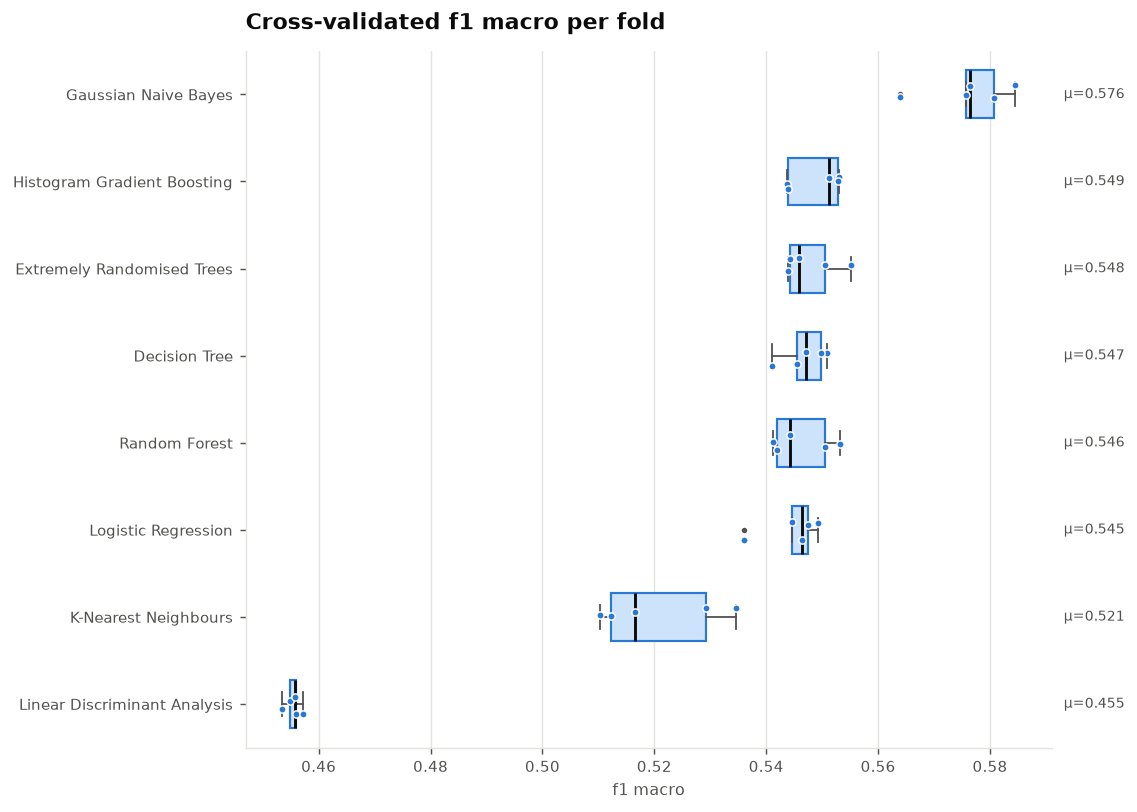
\includegraphics[width=0.92\textwidth]{../docs/figures/cv-macro-f1.png}
\caption{Per-fold macro $F_1$. The spread is the point: a mean without it is
noise. The top model is separated from the field; the six mid-table models are
not separated from one another.}
\end{figure}

\subsection{The accuracy trap, demonstrated}

\keypoint{The last row of Table~\ref{tab:results} is the point of the entire
project. Linear discriminant analysis posts the \textbf{highest accuracy in the
table---$83.0\%$}, nineteen points clear of the best-ranked model---alongside a
balanced accuracy of exactly $0.500$ and an MCC of $-0.010$. Those two numbers
say what accuracy conceals: it predicts ``No'' for all $6{,}110$ hold-out
respondents and has learned nothing whatsoever. Its accuracy is precisely the
majority-class prevalence, because that is what it is.}

$k$-nearest neighbours is halfway down the same road at $0.799$ accuracy and
$0.533$ balanced accuracy: not fully degenerate, but close.

Ranked by accuracy, these two models lead the benchmark. Ranked by any metric
that respects the minority class, they come last. Version~1 of this project
reported accuracy.

\subsection{What the data actually supports}

The honest conclusion is more modest than any single number suggests. The best
macro $F_1$ is $0.576$ against a $0.453$ floor set by the degenerate
classifier---real signal, but weak. Three further observations:

\paragraph{The estimates are stable and unleaked.} Cross-validation and
hold-out macro $F_1$ agree to within $0.01$ for every model ($0.576 \to 0.578$
for the winner), and the fold-to-fold standard deviation is $0.004$--$0.011$. A
leaking pipeline would typically show the hold-out column falling well below
the cross-validation column; it does not.

\paragraph{The ranking is statistically separable at the top.} Paired
$t$-tests put Gaussian Naive Bayes ahead of every rival at $p < 0.005$
($\Delta = +0.027$ against the runner-up, $p = 0.0026$). The gaps
\emph{between} the six mid-table models, by contrast, are $0.001$--$0.003$:
noise.

\paragraph{The metrics disagree about second place, and that is worth
reporting.} Gaussian NB wins macro $F_1$ ($0.578$) but Logistic Regression has
the best MCC ($0.207$) and balanced accuracy ($0.637$). They are making
different trade-offs: NB's hold-out confusion matrix is $3{,}806 / 1{,}266$ on
the majority class and $550 / 488$ on the minority---it keeps majority-class
accuracy high and catches $47\%$ of the minority---whereas Logistic Regression
sacrifices majority accuracy to catch more. Which is preferable is a deployment
question (the cost of a missed case versus a false alarm), not a modelling one,
and the tool's job is to surface the trade-off rather than resolve it silently.

\begin{figure}[htbp]
\centering
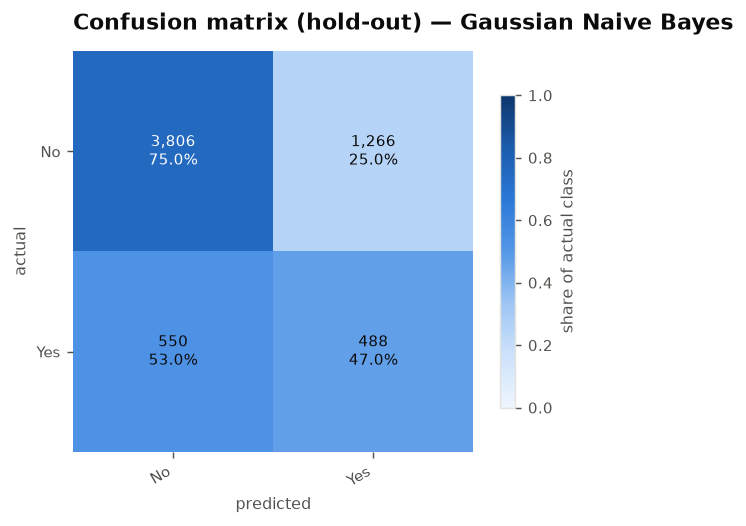
\includegraphics[width=0.66\textwidth]{../docs/figures/confusion-matrix.png}
\caption{Hold-out confusion matrix for the selected model. Counts and
row-normalised shares are printed on every cell, so magnitude never depends on
colour alone.}
\end{figure}

\subsection{Feature importance}

\begin{figure}[htbp]
\centering
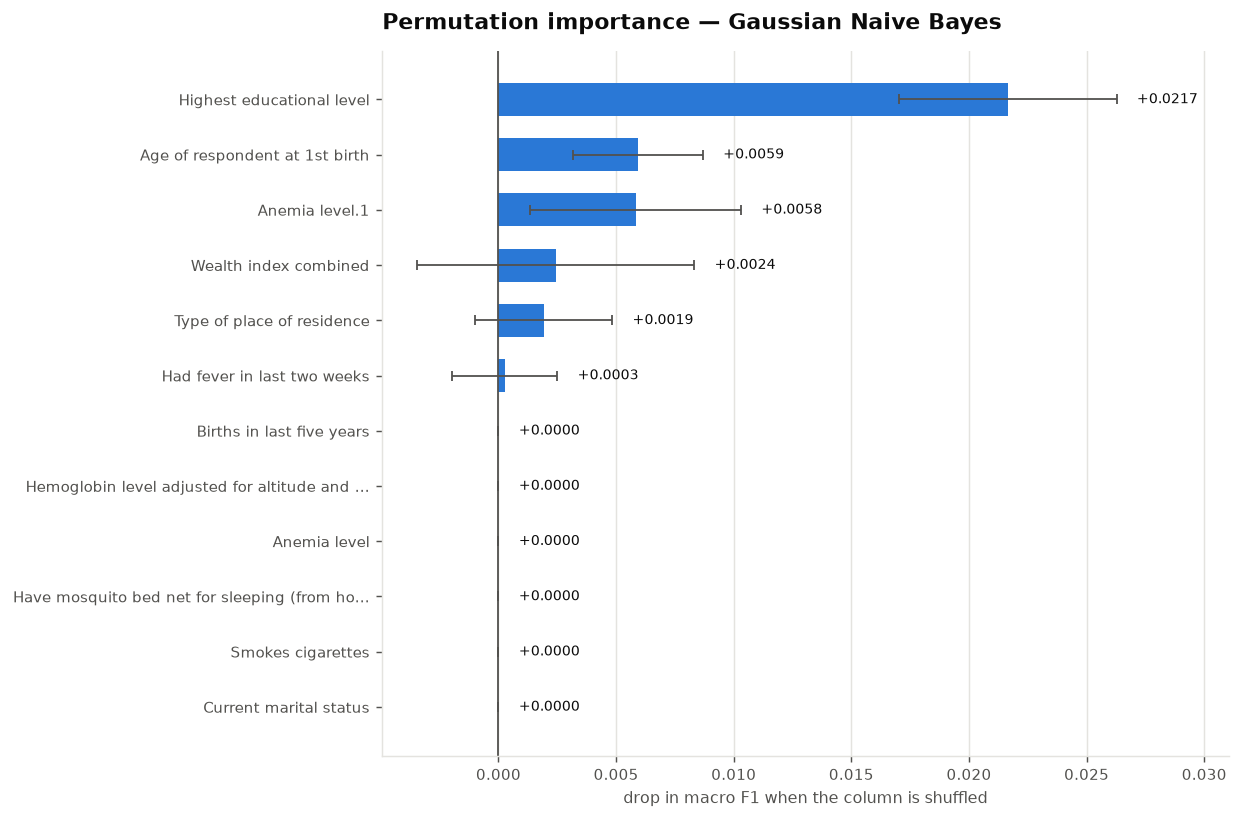
\includegraphics[width=0.94\textwidth]{../docs/figures/permutation-importance.png}
\caption{Permutation importance on held-out data, with the standard deviation
over five repeats. Seven of the twelve inputs are indistinguishable from zero.}
\end{figure}

Permutation importance concentrates the signal in a handful of socio-economic
columns. \textbf{Highest educational level} dominates: shuffling it costs
$0.0217$ macro $F_1$, roughly four times the next column. \textbf{Age at first
birth} ($0.0059$), \textbf{anaemia level} ($0.0058$) and \textbf{wealth index}
($0.0024$) follow, then \textbf{type of residence} ($0.0019$).

Seven of the twelve inputs move the score by less than $0.0005$---within their
own error bars, i.e.\ indistinguishable from noise. This says the 25-feature
budget is generous and a far smaller model would perform identically, which is
a more useful finding than a marginal accuracy gain. The ordering is consistent
with the public-health literature on supplement uptake, where education and
socio-economic status are the dominant determinants.

\subsection{Interpretation}

Socio-economic survey responses carry real but limited information about
supplement uptake. A tool reporting $0.95$ on this dataset would be reporting a
leak, not a discovery. The value of the exercise is that the pipeline makes the
weak-signal conclusion \emph{visible and defensible}: the fold spread is small,
the hold-out confirms the cross-validation, the winning margin is significant,
and the importance analysis explains where the little signal there is comes
from.

% ===========================================================================
\section{Verification of the implementation}
\markboth{Verification}{}

A tool whose selling point is correctness has to demonstrate it. The suite is
\textbf{99 tests, running in about six seconds} on synthetic data, plus
\texttt{ruff} static analysis; both run clean.

\begin{center}
\begin{tabularx}{\textwidth}{L{2.7cm} X}
\toprule
\textbf{Area} & \textbf{Coverage} \\
\midrule
Configuration & validation bounds, JSON round-trip, unknown-key rejection \\
Registries & every scaler, selector, splitter and model builds; every grid targets real parameters; estimators pickle (required for \texttt{n\_jobs > 1}) \\
Data layer & split sizes, stratification, constant / all-missing / high-cardinality / duplicate-header handling, unlabelled-row removal, single-class rejection \\
Evaluation & all metrics collected, signal learned on synthetic data, CV/hold-out agreement, confusion-matrix totals, tuning, importance ranking, comparison ordering \\
End to end & every artefact written and non-empty, the PDF is a real PDF, \texttt{results.json} complete, a run reproduces from its own config \\
CLI & flag mapping, \texttt{-{}-all-models} expansion, target by name or index, clean exit codes on bad input \\
\bottomrule
\end{tabularx}
\end{center}

Four tests exist specifically to pin down the v1 defects:

\begin{center}
\begin{tabularx}{\textwidth}{L{6.6cm} X}
\toprule
\textbf{Test} & \textbf{Guards against} \\
\midrule
\texttt{test\_transformers\_learn\_from\_\-training\_rows\_only} & preprocessing fitted on data outside the training fold \\
\texttt{test\_train\_and\_test\_share\_\-one\_feature\_space} & transformers refitted separately on the hold-out set \\
\texttt{test\_preprocessing\_is\_refit\_\-per\_fold} & transformers fitted once, before cross-validation \\
\texttt{test\_run\_is\_reproducible\_\-from\_its\_own\_config} & results that cannot be regenerated \\
\bottomrule
\end{tabularx}
\end{center}

The first is the interesting one. It fits the pipeline on the training split,
then multiplies every numeric column of the \emph{hold-out} split by $10^{6}$
and refits; the transformed training matrices must be bit-identical. If any
statistic were being drawn from outside the training fold, the corruption would
propagate and the assertion would fail.

% ===========================================================================
\section{Limitations and future work}
\markboth{Limitations}{}

Stated plainly, because a tool that hides its limitations is the problem it
claims to solve.

\begin{center}
\small
\begin{tabularx}{\textwidth}{L{3.5cm} L{4.4cm} X}
\toprule
\textbf{Limitation} & \textbf{Consequence} & \textbf{The principled fix} \\
\midrule
Grouped data unsupported & repeated measurements per subject leak across folds & collect a grouping column and pass it to \texttt{GroupKFold}; the tool currently \emph{refuses} group CV rather than leaking silently \\
Temporal order unverified & \texttt{time\_series} splits assume rows are already ordered & require and validate a timestamp column \\
High-cardinality categoricals dropped & a crude 50-level heuristic discards possibly useful columns & target or ordinal encoding \emph{inside} the pipeline, cross-fitted \\
Probabilities uncalibrated & ROC-AUC is valid, but predicted probabilities should not be read as risks & wrap the final estimator in \texttt{CalibratedClassifierCV} \\
Single hold-out split & the hold-out number is one draw, without a variance estimate & repeated nested cross-validation \\
Re-weighting only & some imbalanced problems benefit from SMOTE-style augmentation & add \texttt{imbalanced-learn}, applied strictly inside the fold \\
Small grids & \texttt{-{}-tune} explores a token search space & random or Bayesian search with a compute budget \\
In-memory only & limited to datasets that fit in RAM & out-of-core loading, or sampling with a stated error bound \\
\bottomrule
\end{tabularx}
\end{center}

Beyond these, two extensions would be natural: model-agnostic explanations
(SHAP values alongside permutation importance) and a learning-curve diagnostic,
which would distinguish ``the model is underfitting'' from ``the data has no
more signal to give''---a question Section 7.5 can currently answer only by
argument.

% ===========================================================================
\section{Conclusion}
\markboth{Conclusion}{}

OmniCLF takes an arbitrary tabular CSV and produces a classification experiment
whose numbers can be defended. The engineering claim is narrow and specific:
leakage is prevented by the structure of the object graph rather than by the
user's discipline, metrics that mislead under class imbalance are reported but
never used for ranking, and every run carries the configuration needed to
reproduce it.

The benchmark makes the case better than the architecture diagram does. On a
survey dataset with an $83\%$ majority class, the model that tops the accuracy
column turns out to have learned nothing at all, while the genuinely best model
reaches a macro $F_1$ of $0.576$---a real but modest result that the tool
reports as modest. The rewrite's contribution is not a higher number. It is
that the number is the right one.

% ===========================================================================
\markboth{References}{}
\begin{thebibliography}{9}
\small
\bibitem{leakage} S.~Kaufman, S.~Rosset and C.~Perlich, ``Leakage in data mining: formulation, detection, and avoidance'', \emph{ACM Transactions on Knowledge Discovery from Data} 6(4), 2012.
\bibitem{esl} T.~Hastie, R.~Tibshirani and J.~Friedman, \emph{The Elements of Statistical Learning}, 2nd ed., Springer, 2009. Ch.~7, \S7.10.2, ``The wrong and right way to do cross-validation''.
\bibitem{mcc} D.~Chicco and G.~Jurman, ``The advantages of the Matthews correlation coefficient (MCC) over F1 score and accuracy in binary classification evaluation'', \emph{BMC Genomics} 21(6), 2020.
\bibitem{varoquaux} G.~Varoquaux and O.~Colliot, ``Evaluating machine learning models and their diagnostic value'', \emph{Machine Learning for Brain Disorders}, Springer, 2023.
\bibitem{breiman} L.~Breiman, ``Random Forests'', \emph{Machine Learning} 45(1), 2001.
\bibitem{sklearn} F.~Pedregosa et al., ``Scikit-learn: Machine Learning in Python'', \emph{Journal of Machine Learning Research} 12, 2011.
\bibitem{permimp} A.~Altmann, L.~Tolo\c{s}i, O.~Sander and T.~Lengauer, ``Permutation importance: a corrected feature importance measure'', \emph{Bioinformatics} 26(10), 2010.
\bibitem{dietterich} T.~G.~Dietterich, ``Approximate statistical tests for comparing supervised classification learning algorithms'', \emph{Neural Computation} 10(7), 1998.
\end{thebibliography}

% ===========================================================================
\appendix
\section{Reproducing every number in this report}
\markboth{Appendix A}{}

\begin{lstlisting}[style=sh]
python -m venv .venv && source .venv/bin/activate
pip install -r requirements.txt

python main.py --models logistic_regression lda naive_bayes knn \
                        decision_tree random_forest extra_trees \
                        hist_gradient_boosting \
               --drop-target-values "Don't know" \
               --selector anova --n-features 25 --n-splits 5 \
               --run-name baseline
\end{lstlisting}

Section 7 is \texttt{runs/baseline/report.pdf}; the per-fold scores are in
\texttt{runs/baseline/results.json}. To replay a run byte-for-byte:

\begin{lstlisting}[style=sh]
python main.py --config runs/baseline/config.json
\end{lstlisting}

Test suite and linter:

\begin{lstlisting}[style=sh]
pip install -r requirements-dev.txt
pytest          # 99 tests
ruff check .
\end{lstlisting}

\section{Command-line reference}
\markboth{Appendix B}{}

\begin{center}
\small
\begin{tabularx}{\textwidth}{L{4.6cm} L{2.9cm} X}
\toprule
\textbf{Flag} & \textbf{Default} & \textbf{Meaning} \\
\midrule
\texttt{-{}-dataset} & \texttt{dataset.csv} & input CSV \\
\texttt{-{}-target} & \texttt{-1} & target column, by name or index \\
\texttt{-{}-drop-columns} & --- & columns to exclude \\
\texttt{-{}-drop-target-values} & --- & label values to discard \\
\texttt{-{}-holdout-size} & \texttt{0.20} & fraction reserved and never trained on \\
\texttt{-{}-scaler} & \texttt{standard} & one of 8 \\
\texttt{-{}-selector} & \texttt{anova} & one of 9 \\
\texttt{-{}-n-features} & \texttt{10} & features requested from the selector \\
\texttt{-{}-models} & \texttt{random\_forest} & one or more classifiers \\
\texttt{-{}-all-models} & --- & benchmark the whole registry \\
\texttt{-{}-cv} & \texttt{stratified\_kfold} & one of 7 \\
\texttt{-{}-n-splits} & \texttt{5} & cross-validation folds \\
\texttt{-{}-tune} & off & grid search inside the training folds \\
\texttt{-{}-no-class-weight} & --- & disable balanced class weights \\
\texttt{-{}-no-importance} & --- & skip permutation importance \\
\texttt{-{}-random-state} & \texttt{42} & seed for split, folds, estimators, permutations \\
\texttt{-{}-n-jobs} & \texttt{-1} & parallel workers \\
\texttt{-{}-output-dir} & \texttt{runs} & where results are written \\
\texttt{-{}-run-name} & timestamp & run directory name \\
\texttt{-{}-config} & --- & replay a saved \texttt{config.json} \\
\texttt{-{}-interactive} & --- & guided prompts (the default with no arguments) \\
\texttt{-{}-list-options} & --- & print every registry entry and exit \\
\bottomrule
\end{tabularx}
\end{center}

\end{document}
